\chapter{巴比倫傾倒，羔羊得勝（17:1-18:24）}

巴比倫代表奢華、權勢與經濟利益引誘世人的世界體系。

約翰看見一個穿著華美、坐在朱紅色獸上的女人，她擁有金子、寶石和珍珠。她與地上的君王聯合，使列國沉醉，也使地上的客商因她的奢華而發財。她華麗的外表之下，隱藏著罪惡、偶像、淫亂、驕傲，以及她對神子民的逼迫。她看似強大、富足、不可撼動，神卻宣告她終必傾倒。

巴比倫最危險的地方，不只是她公開敵對神，而是她具有極大的吸引力。她以財富、成功、權勢、奢華和享樂吸引人，使人以為這就是人生所應追求的榮耀。她不一定要求人立刻否認神；她更可能使人慢慢把安全感放在財富，把價值建立在成功，把盼望寄託在權勢，把滿足建立在物質上。

因此，巴比倫的信息不只是給末世的讀者，也是給今天每一個活在世界中的基督徒。

我們工作、經商、使用金錢、科技和社會資源，是神所賜的美好事物。
而且我們不能離開世界而生活。
問題不是我們是否使用這些東西，而是我們是否開始敬拜這些東西；不是我們是否擁有財富，而是財富是否開始擁有我們的心。
神不是呼召基督徒逃離世界，而是呼召我們不要被世界的價值觀同化。

所以，神對祂的百姓發出一個清楚的呼召：
「我的民哪，你們要從那城出來，免得與她一同有罪。」（啟示錄18:4）

啟示錄把兩個女人放在我們面前：一邊是坐在獸上的巴比倫，一邊是預備自己迎接羔羊的教會；一邊是地上的奢華，一邊是天上的榮耀；一邊看似強大卻轉眼傾倒，一邊在世上似乎軟弱卻永遠屬於得勝的羔羊。

願我們在這個世界中仍然忠心跟隨基督，在誘惑中持守聖潔，在物質的吸引中保持清醒，在地上的權勢面前仍然敬拜那位真正的萬王之王。

\section{巴比倫}

\begin{ScriptureBox}

\item[17:1] 拿著七碗的七位天使中、有一位前來對我說、你到這裡來、我將坐在眾水上的大淫婦所要受的刑罰指給你看．

\item[17:2] 地上的君王與他行淫．住在地上的人喝醉了他淫亂的酒。

\item[17:3] 我被聖靈感動、天使帶我到曠野去．我就看見一個女人騎在朱紅色的獸上．那獸有七頭十角、遍體有褻瀆的名號。

\item[17:4] 那女人穿著紫色和朱紅色的衣服、用金子寶石珍珠為妝飾．手拿金杯、杯中盛滿了可憎之物、就是他淫亂的污穢。

\item[17:5] 在他額上有名寫著說、奧秘哉、大巴比倫、作世上的淫婦和一切可憎之物的母。

\item[17:6] 我又看見那女人喝醉了聖徒的血、和為耶穌作見證之人的血．我看見他、就大大的希奇。

\item[17:7] 天使對我說、你為甚麼希奇呢．我要將這女人和馱著他的那七頭十角獸的奧秘告訴你。

\item[17:8] 你所看見的獸、先前有、如今沒有．將要從無底坑裡上來、又要歸於沉淪。凡住在地上名字從創世以來沒有記在生命冊上的、見先前有、如今沒有、以後再有的獸、就必希奇。

\end{ScriptureBox}


\begin{figure}[htbp]
    \centering
    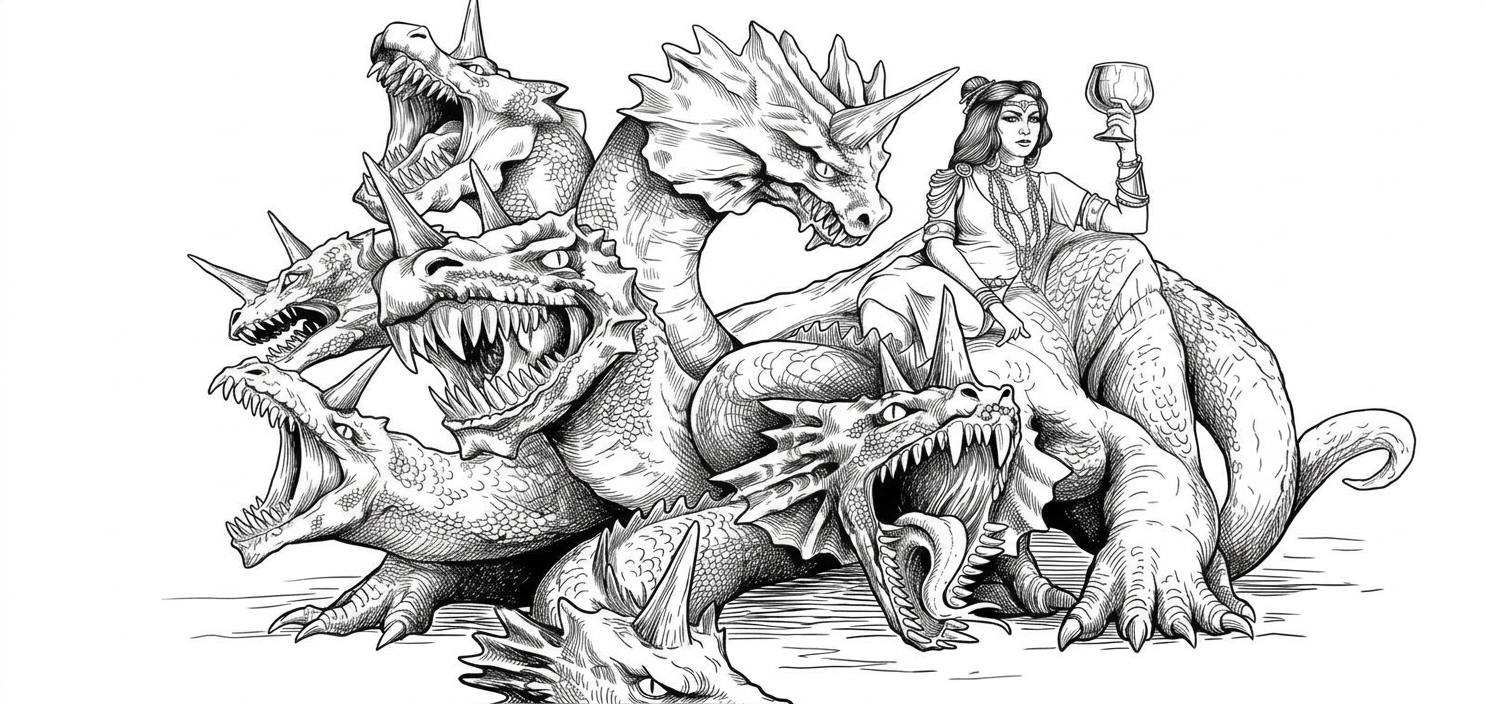
\includegraphics[
    width=1\textwidth, 
    trim=0 0 0 0, 
    clip]{images/babylon_harlot.jpg}
    %\caption{}
    %\label{}
\end{figure}




\begin{ScriptureBox}

\item[17:9] 智慧的心在此可以思想．那七頭就是女人所坐的七座山．

\item[17:10] 又是七位王．五位已經傾倒了、一位還在、一位還沒有來到．他來的時候、必須暫時存留。

\item[17:11] 那先前有、如今沒有的獸、就是第八位．他也和那七位同列、並且歸於沉淪。

\item[17:12] 你所看見的那十角、就是十王．他們還沒有得國．但他們一時之間、要和獸同得權柄與王一樣。

\item[17:13] 他們同心合意、將自己的能力權柄給那獸。

\item[17:14] 他們與羔羊爭戰、羔羊必勝過他們、因為羔羊是萬主之主、萬王之王．同著羔羊的、就是蒙召被選有忠心的、也必得勝。

\item[17:15] 天使又對我說、你所看見那淫婦坐的眾水、就是多民多人多國多方。

\item[17:16] 你所看見的那十角、與獸、必恨這淫婦、使他冷落赤身．又要喫他的肉、用火將他燒盡。

\item[17:17] 因為　神使諸王同心合意、遵行他的旨意、把自己的國給那獸、直等到　神的話都應驗了。

\item[17:18] 你所看見的那女人、就是管轄地上眾王的大城。

\end{ScriptureBox}

「巴比倫」可以解釋成第一世紀的羅馬，或是廣泛的敵對神之世界體系。因此，歷來解經家對「巴比倫」「十王」的具體身分有不同理解。
我列表出對這十王的主要解釋於表\ref{tab:ten-kings-zh} ：

{
\renewcommand{\arraystretch}{1}
\small
\begin{longtable}{p{3.6cm} p{5.4cm}}
\caption{「十王」的不同解釋（啟示錄17章）}
\label{tab:ten-kings-zh} \\
\hline
「十王」的解釋 &
主要依據 \\
\hline
\endfirsthead

\multicolumn{2}{l}{\small\itshape 表~\thetable（續）} \\
\hline
「十王」的解釋 &
主要依據 \\
\hline
\endhead

\hline
\endfoot

\hline
\endlastfoot

末世十個政治勢力的聯盟 &
17:12--13。 \\
第一世紀羅馬歷史中的十位皇帝 &
17:10「五位已經傾倒、一位還在、一位還沒有來到」。 \\
但以理書中的帝國 &
強調但以理書7章四獸與十角的背景。 \\
象徵的政治權勢 &
著重啟示錄的象徵語言，不一定是十位確定的君王。 \\
\end{longtable}
}

無論採取哪一種理解，此章的主要信息都是，這些地上的權勢最終要與羔羊爭戰，但「羔羊必勝過他們，因為羔羊是萬主之主、萬王之王」。

\section{你們要從那城出來、免得與他一同有罪}

\begin{ScriptureBox}

\item[18:1] 此後、我看見另有一位有大權柄的天使從天降下．地就因他的榮耀發光。

\item[18:2] 他大聲喊著說、巴比倫大城傾倒了、傾倒了、成了鬼魔的住處、和各樣污穢之靈的巢穴、〔或作牢獄下同〕並各樣污穢可憎之雀鳥的巢穴。

\item[18:3] 因為列國都被他邪淫大怒的酒傾倒了．地上的君王與他行淫、地上的客商、因他奢華太過就發了財。

\item[18:4] 我又聽見從天上有聲音說、我的民哪、你們要從那城出來、免得與他一同有罪、受他所受的災殃．

\item[18:5] 因他的罪惡滔天他的不義　神已經想起來了。

\item[18:6] 他怎樣待人、也要怎樣待他、按他所行的加倍的報應他．用他調酒的杯、加倍的調給他喝。

\item[18:7] 他怎樣榮耀自己、怎樣奢華、也當叫他照樣痛苦悲哀．因他心裡說、我坐了皇后的位、並不是寡婦、決不至於悲哀。

\item[18:8] 所以在一天之內、他的災殃要一齊來到、就是死亡、悲哀、饑荒、他又要被火燒盡了．因為審判他的主　神大有能力。

\item[18:9] 地上的君王、素來與他行淫一同奢華的、看見燒他的煙、就必為他哭泣哀號．

\item[18:10] 因怕他的痛苦、就遠遠的站著說、哀哉、哀哉、巴比倫大城、堅固的城阿、一時之間你的刑罰就來到了。

\item[18:11] 地上的客商也都為他哭泣悲哀、因為沒有人再買他們的貨物了．

\item[18:12] 這貨物就是金、銀、寶石、珍珠、細麻布、紫色料、綢子、朱紅色料、各樣香木、各樣象牙的器皿、各樣極寶貴的木頭和銅、鐵、漢白玉的器皿、

\item[18:13] 並肉桂、荳蔻、香料、香膏、乳香、酒、油、細麵、麥子、牛、羊、車、馬、和奴僕、人口。

\item[18:14] 巴比倫哪、你所貪愛的果子離開了你．你一切的珍饈美味、和華美的物件、也從你中間毀滅、決不能再見了。

\item[18:15] 販賣這些貨物、藉著他發了財的客商、因怕他的痛苦、就遠遠的站著哭泣悲哀、說、

\item[18:16] 哀哉、哀哉、這大城阿、素常穿著細麻、紫色、朱紅色的衣服、又用金子、寶石、和珍珠為妝飾．

\item[18:17] 一時之間、這麼大的富厚就歸於無有了。凡船主、和坐船往各處去的、並眾水手、連所有靠海為業的、都遠遠的站著、

\item[18:18] 看見燒他的煙、就喊著說、有何城能比這大城呢。

\item[18:19] 他們又把塵土撒在頭上、哭泣悲哀、喊著說、哀哉、哀哉、這大城阿．凡有船在海中的、都因他的珍寶成了富足．他在一時之間就成了荒場。

\item[18:20] 天哪、眾聖徒眾使徒眾先知阿、你們都要因他歡喜．因為　神已經在他身上伸了你們的冤。

\item[18:21] 有一位大力的天使舉起一塊石頭、好像大磨石、扔在海裡、說、巴比倫大城、也必這樣猛力的被扔下去、決不能再見了。

\item[18:22] 彈琴、作樂、吹笛、吹號的聲音、在你中間決不能再聽見．各行手藝人在你中間決不能再遇見．推磨的聲音在你中間決不能再聽見．

\item[18:23] 燈光在你中間決不能再照耀．新郎和新婦的聲音、在你中間決不能再聽見．你的客商原來是地上的尊貴人．萬國也被你的邪術迷惑了。

\item[18:24] 先知和聖徒、並地上一切被殺之人的血、都在這城裡看見了。

\end{ScriptureBox}

地上的君王和客商看到一天之內就傾倒焚毀的巴比倫城，他們就為城哭泣哀號。
這已經是七印、七號、七碗最頂峰，他們自己隨時可以滅亡。可是他們哭泣，竟然不是為了自己，而是為了所有的財寶。
可見他們貪戀財寶的心，已經使他們忘了在大審判時自身的性命安危，只是為了財寶哭泣。


\begin{figure}[htbp]
    \centering
    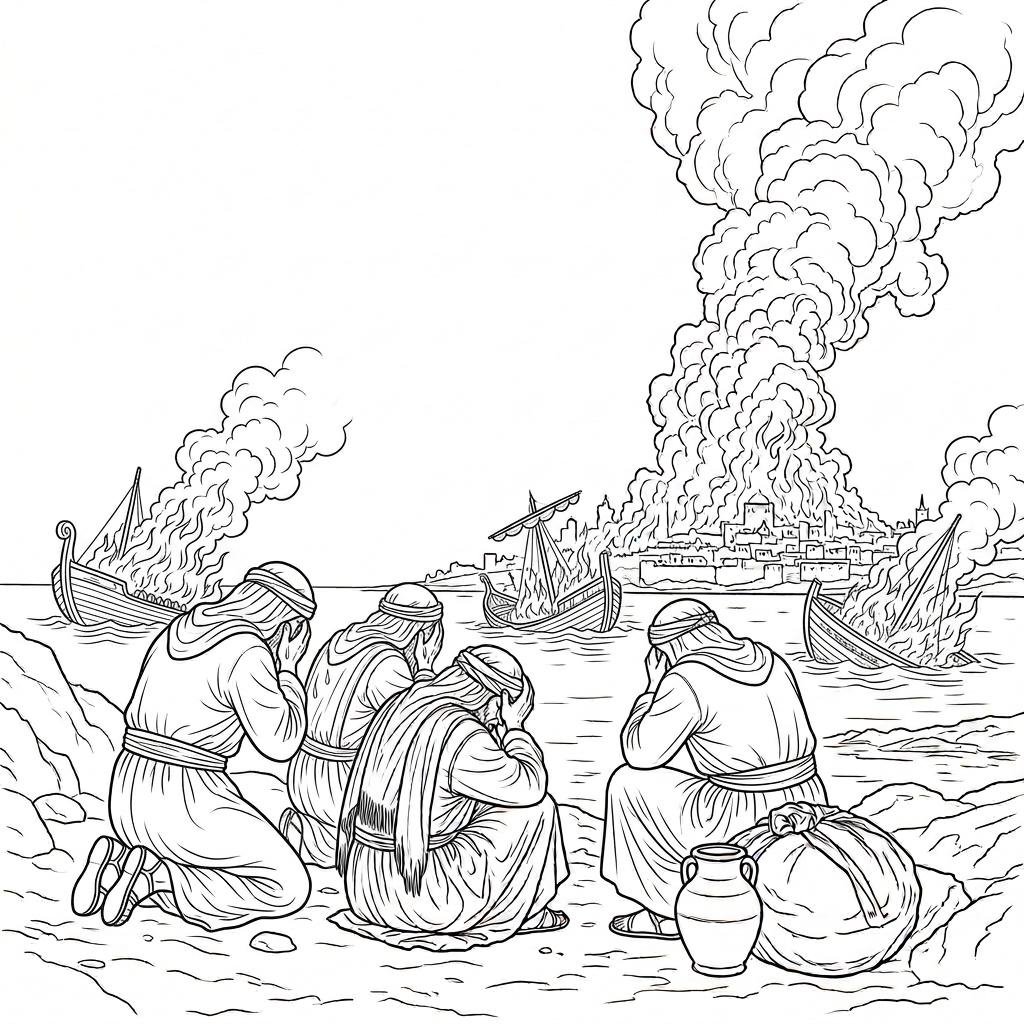
\includegraphics[
    width=1\textwidth, 
    trim=0 0 0 0, 
    clip]{images/rev_18_bablyon_burning.jpg}
    %\caption{}
    %\label{}
\end{figure}





獸代表敵對神的權勢，十角代表與獸聯合的十王，巴比倫以及大淫婦則象徵以奢華、權勢與經濟利益迷惑列國的世界體系。他們因共同的利益而聯合，將權柄交給獸，並一同敵對羔羊。最後，十角與獸反過來恨惡淫婦，使她荒涼、赤身，並焚燒她。這顯明敵對神的勢力雖能暫時結盟，卻不是永遠穩固的。神仍然掌管歷史，甚至使用他們彼此反目來成就祂的審判。

對初代教會而言，巴比倫的異象是當時信徒所面對的信仰抉擇。
因為羅馬掌握強大的政治權力，擁有龐大的商業網絡與豐富的物質資源，也以皇帝崇拜等方式彰顯其權威。
然而，當社會要求他們參與偶像崇拜，或以不符合信仰的方式表達對皇帝與地上權勢的忠誠時，他們就必須作出選擇：究竟要順從當時的社會要求，還是忠於耶穌基督？

相對於18章的巴比倫的淫婦，啟示錄21章的羔羊的新婦更是無以倫比。表\ref{tab:babylon_bride} 就顯出此對照。

{
\begin{center}
\small
\label{tab:babylon_bride}
\renewcommand{\arraystretch}{1}
\begin{longtable}{p{0.8cm} p{4.1cm} p{4.1cm}}
\caption{聖城的新婦無以倫比} \\
\hline
對比 & 巴比倫的淫婦（18章） & 聖城的新婦（21章） \\
\hline
經文 & 17:1-6；18:1-24 & 21:2, 9-10 \\

象徵 & 迷惑列國的世界體系。 & 神的子民，蒙羔羊救贖。 \\

外在 & 穿紫色和朱紅色衣服，裝飾金子、寶石、珍珠。 & 城中有神的榮耀，光輝如極貴的寶石。（11） \\

列國關係 & 地上的君王與她行淫。 & 地上的君王將榮耀歸與城（24-26） \\

與神關係 & 充滿可憎之物，並流了聖徒的血。 & 神的帳幕在人間，神要與人同住（3） \\

與人關係 & 客商因她的奢華發財。（3, 15-19） & 神白白賜生命水給口渴的人（6, 17） \\

眼淚與死亡 & 世上的人因她的毀滅而哀哭。（9-19） & 神要擦去人的眼淚，不再有死亡、悲哀、哭號、疼痛（4） \\
結局 & 毀滅（8-10, 21） & 從天而降，永遠與神同住（2-3） \\

\hline
\end{longtable}
\end{center}
}

\section*{小組討論題}

\begin{enumerate}
    \item 巴比倫外表華美、富足，卻充滿罪惡並逼迫聖徒。這個對比如何提醒我們，不要只憑外在的繁榮判斷一個社會或體系？

    \item 神說：「我的民哪，你們要從那城出來，免得與她一同有罪。」這句話對初代教會有什麼意義？對今日教會又有什麼提醒？

    \item 今天的信徒可能在哪些方面受到巴比倫的價值觀吸引？例如財富、成功、權勢、享樂或人的肯定。我們如何察驗自己的心？


\end{enumerate}
